%\documentclass[12pt]{scrreprt}
\documentclass[12pt]{report}

% language may be romanian or english (default is english)
% type may be bachelor or master (default is bachelor)
\usepackage[language=english, type=master]{style}

%\geometry{a4paper,top=2.5cm,left=3cm,right=2.5cm,bottom=2.5cm}
%in style
%controlling the appearance of your headers and footers
\usepackage{fancyhdr}
\usepackage{amsmath}
\usepackage{amssymb}
\pagestyle{fancy}
\lhead{}
\chead{}
\renewcommand{\headrulewidth}{0.2pt}
\renewcommand{\footrulewidth}{0.2pt}

\begin{document}

% ============================================================================
% ENGLISH TITLE PAGE
% ============================================================================
\begin{titlepage}
\begin{center}
{\Large\textbf{BABEŞ-BOLYAI UNIVERSITY CLUJ-NAPOCA}\\[1em]
\textbf{FACULTY OF MATHEMATICS AND COMPUTER SCIENCE}\\[1em]
\textbf{SPECIALIZATION: ADVANCED INFORMATION SYSTEMS}}
\end{center}

\vspace{8em}

\begin{center}
    \Huge\textbf{MASTER'S THESIS}
\end{center}

\vspace{2em}

\begin{center}
    \Large\textbf{Efficient Inter-Process Communication with Zero-Copy Semantics:\\[0.5em] A Rust-Based Shared Memory Library for Python}
\end{center}

\vspace{9em}

\begin{flushleft}
{\Large\textbf{Scientific Supervisor \\ Lect. Dr. Eng. Bența Kuderna-Iulian}}
\end{flushleft}

\vspace{3em}

\begin{flushright}
{\Large\textit{Absolvent\\ Filea Răzvan-Gheorghe}}
\end{flushright}

\vfill

\begin{center}
{\Large{2026}}
\end{center}
\end{titlepage}

% ============================================================================
% GERMAN TITLE PAGE
% ============================================================================
\begin{titlepage}
\begin{center}
{\Large\textbf{BABEŞ-BOLYAI UNIVERSITÄT CLUJ-NAPOCA}\\[1em]
\textbf{FAKULTÄT FÜR MATHEMATIK UND INFORMATIK}\\[1em]
\textbf{SPEZIALISIERUNG: FORTGESCHRITTENE INFORMATIONSSYSTEME}}
\end{center}

\vspace{10em}

\begin{center}
    \Huge\textbf{MASTERARBEIT}
\end{center}

\vspace{2em}

\begin{center}
    \Large\textbf{Effiziente Interprozesskommunikation mit Zero-Copy-Semantik:\\[0.5em] Eine Rust-basierte Shared-Memory-Bibliothek für Python}
\end{center}

\vspace{7em}

\begin{flushleft}
{\Large\textbf{Wissenschaftlicher Betreuer \\ Lekt. Dr. Ing. Bența Kuderna-Iulian}}
\end{flushleft}

\vspace{3em}

\begin{flushright}
{\Large\textit{Absolvent\\ Filea Răzvan-Gheorghe}}
\end{flushright}

\vfill

\begin{center}
{\Large{2026}}
\end{center}
\end{titlepage}

% ============================================================================
% ROMANIAN TITLE PAGE
% ============================================================================
\begin{titlepage}
\begin{center}
{\Large\textbf{UNIVERSITATEA BABEŞ-BOLYAI CLUJ-NAPOCA}\\[1em]
\textbf{FACULTATEA DE MATEMATICĂ ŞI INFORMATICĂ}\\[1em]
\textbf{SPECIALIZAREA: SISTEME INFORMATICE AVANSATE}}
\end{center}

\vspace{10em}

\begin{center}
    \Huge\textbf{LUCRARE DE DISERTAŢIE}
\end{center}

\vspace{2em}

\begin{center}
    \Large\textbf{Comunicare Eficientă între Procese cu Semantică Zero-Copy:\\[0.5em] O Bibliotecă Bazată pe Rust pentru Comunicare prin Memorie Partajată în Python}
\end{center}

\vspace{7em}

\begin{flushleft}
{\Large\textbf{Conducător ştiinţific \\ Lect. Dr. Ing. Bența Kuderna-Iulian}}
\end{flushleft}

\vspace{3em}

\begin{flushright}
{\Large\textit{Absolvent\\ Filea Răzvan-Gheorghe}}
\end{flushright}

\vfill

\begin{center}
{\Large{2026}}
\end{center}
\end{titlepage}

\newpage
\thispagestyle{empty}
\mbox{}
\newpage
\pagenumbering{roman}

\cleardoublepage
\textbf{ABSTRACT}
\vspace{0.5cm}
\hrule
\vspace{0.5cm}
%\cleardoublepage

Python's native inter-process communication mechanisms exhibit significant performance limitations in data-intensive applications requiring low-latency data transfer. This thesis presents \texttt{rs\_ipc}, a high-performance IPC library implemented in Rust that achieves zero-copy communication through POSIX shared memory.

The library introduces a \texttt{SharedMessage} abstraction with futex-based synchronization, enabling efficient producer-consumer patterns without pthread FFI overhead. Key design features include direct shared memory access eliminating redundant copies, version checking without lock acquisition, flexible blocking strategies (non-blocking, partial-blocking, full-blocking), and GIL-free operations for Python multithreading.

Benchmarks across embedded platforms and workstations demonstrate significant speedups over Python's \texttt{multiprocessing} primitives. The partial-blocking communication strategy enables faster processing pipelines to proceed without waiting on slower ones, substantially improving overall throughput in concurrent applications. Validation on a 1:10 scale autonomous vehicle confirms applicability to real-time computer vision systems.


\tableofcontents


\newpage
\pagenumbering{arabic}

\chapter{Introduction}
\label{chap:intro}

\section{Context and Motivation}

Python's Global Interpreter Lock (GIL) prevents multiple threads from executing Python bytecode simultaneously, forcing CPU-bound workloads into a multiprocessing architecture where separate processes must exchange data through inter-process communication. Python's dominance in data-intensive domains---computer vision, machine learning, scientific computing---means these systems frequently require the kind of concurrent, low-latency data transfer that Python's standard library was never designed to provide.

For applications that transfer large payloads---video frames of several megabytes, NumPy tensors, or serialized model states---the performance of this communication layer determines overall system throughput. A vision pipeline processing 30 frames per second at 2.6\,MiB per pipeline message (e.g., multiple sensor arrays per processing stage), for instance, generates over 78\,MiB/s of IPC traffic per producer-consumer pair; with multiple consumers, aggregate bandwidth demands quickly exceed what Python's standard library mechanisms can deliver efficiently.

Yet Python's built-in IPC primitives were designed for generality rather than performance. They impose serialization overhead, redundant memory copies, or require developers to manually implement synchronization over raw shared memory. The gap between what these mechanisms provide and what performance-critical applications require motivates the design of a purpose-built library: one that eliminates unnecessary copies, minimizes synchronization overhead, and exposes flexible producer-consumer policies suited to diverse communication topologies.

\newpage
\section{Problem Statement}
\label{sec:problem_statement}

Python's standard library offers several IPC mechanisms, each with significant limitations for high-performance applications:

\begin{itemize}
    \item \textbf{multiprocessing.Pipe}: Provides bidirectional communication but requires serialization (pickling) of data. For large objects, the serialization overhead and memory copies impose substantial latency.

    \item \textbf{multiprocessing.Queue}: Built on pipes with an internal feeder thread, this mechanism requires full serialization (pickling) of data and transfers it through kernel-mediated pipe buffers, combining serialization overhead with memory copy costs.

    \item \textbf{multiprocessing.shared\_memory}: Introduced in Python 3.8, this module provides raw shared memory access but lacks built-in synchronization. Developers must implement their own locking mechanisms, and Python's lack of cross-process atomic operations complicates safe concurrent access.
\end{itemize}

Furthermore, Python's synchronization primitives exhibit limitations when used across processes. The \texttt{multiprocessing.Lock} cannot be stored in shared memory and must be passed through the parent-child process relationship. Condition variables are conflated with locks, preventing the efficient use of separate read and write notifications. These constraints make it difficult to implement sophisticated producer-consumer patterns efficiently in pure Python.

\bigskip
\section{Proposed Solution}

This thesis presents \texttt{rs\_ipc}, a high-performance inter-process communication library that addresses these limitations through a hybrid Python-Rust architecture. The library provides a \texttt{SharedMessage} abstraction built on POSIX shared memory primitives (\texttt{shm\_open}, \texttt{mmap}), offering:

\begin{itemize}
    \item \textbf{Zero-copy semantics}: Processes read and write directly to shared memory, eliminating the serialization and memory copy overhead inherent in pipe-based communication.

    \item \textbf{Futex-based synchronization}: Direct Linux futex system calls replace pthread FFI, reducing latency and simplifying cross-process synchronization.

    \item \textbf{Flexible blocking strategies}: Support for non-blocking, partial-blocking, and full-blocking communication modes enables adaptation to diverse application requirements.

    \item \textbf{GIL-free operations}: Rust's thread safety guarantees allow blocking IPC operations to release Python's GIL, enabling true concurrency in multithreaded Python applications.
\end{itemize}

By implementing the performance-critical components in Rust and exposing them through PyO3 bindings, the library combines Python's accessibility with systems-level performance.

\bigskip
\section{Contributions}

The primary contributions of this thesis are:

\begin{enumerate}
    \item \textbf{SharedMessage abstraction}: A cache-aligned shared memory data structure with bit-packed atomic fields for efficient producer-consumer communication.

    \item \textbf{Futex-based synchronization primitives}: Custom mutex and condition variable implementations using raw futex system calls, avoiding pthread FFI overhead.

    \item \textbf{Partial-blocking communication}: A novel blocking strategy where producers wait for a configurable subset of consumers, balancing throughput and consistency.

    \item \textbf{Asynchronous operation modes with safe GIL release}: Background threads for non-blocking read and write operations, with demonstrated techniques for releasing Python's GIL during Rust operations while maintaining memory safety.

    \item \textbf{Comprehensive benchmarking}: Performance evaluation comparing against six alternative backends---including ZeroMQ and POSIX IPC---across four communication topologies, with statistical methodology based on multiple independent trials.
\end{enumerate}

The \texttt{rs\_ipc} library originated in a conference paper~\cite{szilagyi2025accelerating} that introduced the initial SharedMessage specification and validated it on a 1:10 scale autonomous vehicle. The present thesis makes three novel contributions beyond the conference paper: (1) redesigned synchronization primitives---replacing the mutex-associated condition variable with a standalone counter-based design that enables lock-free reader waits, and switching from the \texttt{linux-futex} crate to direct syscalls via \texttt{rustix} for full spin-then-block control; (2) a partial-blocking communication policy that enables runtime-configurable producer-consumer delivery guarantees; and (3) a comprehensive performance evaluation against six alternative backends with statistical methodology. Additionally, the thesis introduces engineering improvements including a redesigned cache-aligned memory layout, bit-packed atomic coordination fields, asynchronous operation modes, and safe GIL release patterns for Python integration.

\bigskip
\section{Thesis Structure}

The remainder of this thesis is organized as follows:

\textbf{Chapter~\ref{chap:ch2}} provides the theoretical foundations necessary to understand the implementation. This includes an overview of POSIX shared memory, memory-mapped I/O, synchronization primitives, and the Linux futex subsystem.

\textbf{Chapter~\ref{chap:ch3}} surveys related work in high-performance IPC, including message-passing frameworks, shared memory libraries, and serialization systems, positioning \texttt{rs\_ipc} within the existing landscape.

\textbf{Chapter~\ref{chap:ch4}} details the architecture and implementation of the \texttt{rs\_ipc} library. This chapter covers the \texttt{SharedMessage} data structure, the custom synchronization primitives, the PyO3 integration layer, and the asynchronous operation modes.

\textbf{Chapter~\ref{chap:ch5}} presents the performance evaluation methodology and results. Benchmarks compare the library against Python's native IPC mechanisms across various data sizes and hardware configurations.

\textbf{Chapter~\ref{chap:conclusions}} summarizes the contributions, discusses limitations, and identifies directions for future work.


\chapter{Foundations and Requirements}
\label{chap:ch2}

This chapter presents the theoretical foundations underlying the design and implementation of the \texttt{rs\_ipc} library. Each section introduces a concept or mechanism that is directly utilized in the architecture described in Chapter~\ref{chap:ch3}: POSIX shared memory provides the transport layer, synchronization primitives ensure data consistency, Linux futexes enable efficient cross-process locking, Python's concurrency model motivates the GIL release strategy, and Rust's type system guarantees memory safety across the foreign function boundary.

\section{POSIX Shared Memory and Memory Mapping}
\label{sec:shm}

Shared memory represents the fastest form of inter-process communication available on modern operating systems. Unlike pipe-based or socket-based mechanisms, shared memory allows multiple processes to access the same physical memory region without copying data through the kernel. This section describes the POSIX interfaces that enable this capability.

\subsection{Shared Memory Objects}

The POSIX shared memory API provides two primary functions for managing shared memory objects: \texttt{shm\_open} and \texttt{shm\_unlink}~\cite{posix2017}. The \texttt{shm\_open} function creates or opens a named shared memory object, returning a file descriptor that can be used with standard file operations. On Linux, these objects reside in a \texttt{tmpfs} filesystem mounted at \texttt{/dev/shm}, backed entirely by RAM and swap rather than persistent storage.

The lifecycle of a shared memory object follows a create-size-map-use-unmap-unlink pattern:

\begin{enumerate}
    \item \texttt{shm\_open} creates the object and returns a file descriptor.
    \item \texttt{ftruncate} sets the size of the memory region.
    \item \texttt{mmap} maps the region into the process address space.
    \item Processes read and write directly to the mapped region.
    \item \texttt{munmap} removes the mapping from the process.
    \item \texttt{shm\_unlink} removes the named object from the filesystem.
\end{enumerate}

Named shared memory objects persist in the filesystem namespace until explicitly unlinked, independent of the processes that created them. This property enables communication patterns where the producer and consumer processes do not share a parent-child relationship, unlike anonymous mappings created via \texttt{fork}.

\subsection{Memory-Mapped I/O}

The \texttt{mmap} system call maps a file descriptor (including shared memory objects) into the virtual address space of the calling process~\cite{kerrisk2010}. When invoked with the \texttt{MAP\_SHARED} flag, modifications made by one process become visible to all other processes that have mapped the same underlying object. The kernel ensures coherence through the page table mechanism: all mappings of the same physical page share the same underlying memory, so writes are immediately visible without explicit synchronization at the memory level.

However, visibility at the memory level does not imply ordering guarantees at the instruction level. Modern processors may reorder memory operations for performance, meaning that a write performed by one process may not be observed in the expected order by another process. This gap between memory coherence and memory consistency motivates the synchronization mechanisms described in Section~\ref{sec:sync}.

\subsection{Translation Lookaside Buffer Considerations}

When a process accesses a mapped memory region, the CPU must translate virtual addresses to physical addresses. The Translation Lookaside Buffer (TLB) caches recent translations to avoid costly page table walks. With the default page size of 4~KiB on x86\_64 architectures, a 4~MiB shared memory region spans 1024 pages, each requiring a TLB entry for efficient access.

For large data transfers---such as video frames or tensor buffers---the number of required TLB entries may exceed the available capacity, causing TLB misses that degrade performance. Explicit huge pages (2~MiB or 1~GiB on x86\_64) reduce this pressure by covering larger address ranges with fewer entries. However, explicit huge pages require memory backed by \texttt{hugetlbfs}, which is incompatible with POSIX shared memory objects created via \texttt{shm\_open}. The alternative---Linux Transparent Huge Pages (THP)---can be requested via \texttt{madvise} with the \texttt{MADV\_HUGEPAGE} hint, but the kernel treats this as advisory: allocation depends on the availability of contiguous physical memory and is not guaranteed~\cite{kerrisk2010}. In practice, THP is unreliable for shared memory regions that are frequently created and destroyed, limiting its applicability to long-lived mappings with favorable allocation timing.

\subsection{Shared Memory versus Message Passing}

The fundamental trade-off between shared memory and message-passing IPC lies in the division of responsibility. Message-passing mechanisms (pipes, sockets, message queues) handle serialization, buffering, and delivery on behalf of the application, introducing at least one memory copy per transfer---from the sender's buffer into kernel space, and from kernel space into the receiver's buffer. Shared memory eliminates these copies entirely: both processes operate on the same physical memory, achieving true zero-copy semantics.

The cost of this efficiency is complexity. Shared memory provides no inherent ordering, synchronization, or notification mechanism. The application must explicitly coordinate access to prevent data races, detect when new data is available, and ensure that readers do not observe partially written messages. These requirements motivate the synchronization primitives described in the following section.


\section{Synchronization Primitives}
\label{sec:sync}

When multiple processes share a memory region, concurrent access to the same data without coordination leads to data races: outcomes that depend on the relative timing of operations across processes. This section introduces the synchronization mechanisms that prevent such races, ordered from hardware-level primitives to higher-level abstractions.

\subsection{Atomic Operations}
\label{subsec:atomics}

Modern processors provide instructions that execute indivisibly with respect to other cores. These atomic operations form the foundation of all higher-level synchronization~\cite{herlihy2012}. The two most relevant to this work are Compare-And-Swap (CAS), which conditionally updates a memory location only if it holds an expected value, and Fetch-And-Add, which atomically increments a value and returns the previous one. CAS enables the fast path of lock acquisition (attempting to claim an uncontended lock without kernel involvement), while Fetch-And-Add drives sequence counters and notification mechanisms where multiple writers must produce distinct values without coordination.

\subsection{Memory Ordering}
\label{subsec:memory_ordering}

Atomic operations alone do not suffice for correct synchronization. Modern CPUs and compilers reorder memory operations to improve throughput, subject to per-thread consistency but not cross-thread visibility guarantees. Memory ordering constraints specify how operations on atomic variables relate to operations on other memory locations~\cite{herlihy2012}.

The C++11 memory model, adopted by Rust through its \texttt{std::sync::atomic} module, defines several ordering levels:

\begin{itemize}
    \item \textbf{Relaxed}: No ordering guarantees beyond atomicity. The operation cannot be torn (partially observed), but surrounding reads and writes may be reordered freely. Suitable for counters where only the final value matters.

    \item \textbf{Acquire}: When a load operation uses Acquire ordering, it guarantees that all subsequent reads and writes (in program order) will observe effects that were visible before the corresponding Release store. Conceptually, it ``acquires'' the data published by a Release.

    \item \textbf{Release}: When a store operation uses Release ordering, it guarantees that all preceding reads and writes (in program order) are visible to any thread that performs an Acquire load of the same atomic variable. Conceptually, it ``releases'' or publishes accumulated state.

    \item \textbf{SeqCst} (Sequentially Consistent): The strongest ordering, establishing a single total order of all SeqCst operations across all threads. This prevents subtle reordering issues but limits hardware optimization.
\end{itemize}

The Acquire-Release pair is fundamental to producer-consumer patterns: a producer writes data and then performs a Release store to a flag variable; a consumer performs an Acquire load of the same flag and is guaranteed to observe the producer's data writes. This pattern appears directly in the version-checking mechanism of the \texttt{SharedMessage} implementation.

\subsection{Cache Coherence and False Sharing}
\label{subsec:false_sharing}

Multi-core processors maintain cache coherence through protocols such as MESI (Modified, Exclusive, Shared, Invalid)~\cite{herlihy2012}. When one core modifies a cache line, the protocol invalidates copies held by other cores, forcing them to re-fetch the updated data from a shared cache level or main memory.

Cache coherence operates at the granularity of cache lines, typically 64 bytes on x86\_64 processors. This granularity introduces a subtle performance pathology known as \textit{false sharing}: when two logically independent variables reside on the same cache line, a write to one variable invalidates the other variable's cache entry on remote cores, even though the second variable was not modified.

In the context of shared memory IPC, false sharing is particularly damaging. Consider a structure where a write-mostly field (such as a sequence counter incremented by the producer) and a read-mostly field (such as a consumer count) occupy the same cache line. Every producer write would invalidate the cache line on all consumer cores, forcing them to re-fetch data they are only reading---not because the data changed, but because an adjacent field did.

The standard mitigation is to separate frequently accessed fields into distinct cache lines through explicit padding. Using 128-byte separation (two cache lines) provides additional protection against hardware prefetching, which may speculatively load adjacent cache lines.

\subsection{Mutexes}
\label{subsec:mutexes}

A mutex (mutual exclusion lock) ensures that at most one thread or process executes a critical section at any given time. Conceptually, a mutex provides two operations: \texttt{lock} (acquire exclusive access, blocking if unavailable) and \texttt{unlock} (release exclusive access, potentially waking a blocked waiter).

Mutex implementations occupy a spectrum between two extremes:

\begin{itemize}
    \item \textbf{Spin locks}: The acquiring thread repeatedly tests the lock state in a tight loop. This avoids the overhead of context switches but wastes CPU cycles during contention. Spin locks perform well when critical sections are short and contention is rare.

    \item \textbf{Blocking locks}: When the lock is unavailable, the acquiring thread yields the CPU to the operating system scheduler. This eliminates busy-waiting but incurs the cost of context switches (typically 1--10 microseconds). Blocking locks are appropriate when critical sections are long or contention is frequent.
\end{itemize}

A hybrid approach combines both strategies: spin briefly (optimistic that the lock will be released quickly), then fall back to blocking if the spin phase fails. This approach, described in detail in Section~\ref{sec:futex}, forms the basis of the futex-based lock used in \texttt{rs\_ipc}.

\subsection{Condition Variables}
\label{subsec:condvars}

While mutexes protect shared state, they do not provide a mechanism for threads to efficiently wait for state changes. A thread that needs to wait for a particular condition (e.g., ``new data is available'') could repeatedly acquire the lock, check the condition, release the lock, and retry---a pattern called busy-waiting that wastes CPU resources.

Condition variables solve this problem by allowing a thread to atomically release a lock and suspend execution until another thread signals that the condition may have changed. The fundamental operations are:

\begin{itemize}
    \item \textbf{wait(lock, condition)}: Atomically releases the lock and suspends the calling thread. When the thread is awakened, it re-acquires the lock before returning.

    \item \textbf{notify\_one}: Wakes one suspended thread waiting on the condition variable.

    \item \textbf{notify\_all}: Wakes all suspended threads waiting on the condition variable.
\end{itemize}

In a producer-consumer system, the producer signals the condition variable after writing new data, waking consumers that were waiting for fresh input. The atomicity of the release-and-suspend operation in \texttt{wait} prevents a race condition where a notification arrives between releasing the lock and entering the wait state (the ``lost wakeup'' problem).


\section{The Linux Futex Subsystem}
\label{sec:futex}

Traditional Unix synchronization primitives such as System~V semaphores require a system call for every lock and unlock operation, regardless of whether contention exists. The POSIX threads (pthread) library improves upon this with userspace fast paths, but its use across process boundaries introduces complexity: \texttt{pthread\_mutex\_t} must be initialized with the \texttt{PTHREAD\_PROCESS\_SHARED} attribute, placed in shared memory, and accessed through the same library version in all processes.

The \textit{futex} (Fast Userspace Mutex) subsystem, introduced in Linux 2.5.7~\cite{franke2002}, provides a more fundamental building block that addresses these limitations.

\subsection{Architecture}

A futex operates on a single 32-bit integer in userspace memory. The kernel associates a wait queue with the physical address of this integer, enabling cross-process synchronization without any shared library state. The two core operations are:

\begin{itemize}
    \item \texttt{futex\_wait(addr, expected)}: If the value at \texttt{addr} equals \texttt{expected}, the calling thread is added to the kernel wait queue and suspended. If the values differ, the call returns immediately. This atomic check-and-sleep prevents lost wakeups.

    \item \texttt{futex\_wake(addr, count)}: Wakes up to \texttt{count} threads waiting on the queue associated with \texttt{addr}.
\end{itemize}

The critical insight is that the common case---acquiring an uncontended lock---requires only a userspace atomic CAS operation with no system call. The kernel is involved only when a thread must actually sleep (contended lock) or wake a sleeper (unlock with waiters). This asymmetry makes futexes highly efficient for workloads where contention is infrequent.

\subsection{The Three-State Lock Pattern}

Drepper~\cite{drepper2005} describes an efficient mutex implementation using three states rather than the naive two-state (locked/unlocked) approach:

\begin{itemize}
    \item \textbf{State 0 (Unlocked)}: The lock is available.
    \item \textbf{State 1 (Locked, no waiters)}: The lock is held but no other thread is waiting for it.
    \item \textbf{State 2 (Locked, with waiters)}: The lock is held and at least one thread is blocked in the kernel waiting for it.
\end{itemize}

The distinction between states 1 and 2 is an optimization. When unlocking from state 1, the implementation knows that no threads are waiting and can skip the \texttt{futex\_wake} system call entirely. Only when unlocking from state 2 must the implementation invoke the kernel to wake a waiter. This optimization eliminates a system call on every uncontended unlock operation.

The lock acquisition sequence follows:

\begin{enumerate}
    \item Attempt a CAS from state 0 to state 1 (fast path, no syscall).
    \item If the CAS fails, spin briefly with relaxed loads, hoping the lock is released quickly.
    \item If spinning fails, transition the state to 2 (signaling that waiters exist) and call \texttt{futex\_wait}.
    \item Upon waking, retry acquisition from step 1.
\end{enumerate}

The spin phase (step 2) uses relaxed loads rather than CAS operations to avoid generating cache-line invalidations during the spin. This reduces coherence traffic when multiple threads contend for the same lock.

\subsection{Cross-Process Synchronization}

A key property of the futex subsystem is that wait queues are keyed by physical memory address, not by virtual address or process identity~\cite{franke2002}. Because \texttt{mmap} with \texttt{MAP\_SHARED} causes distinct virtual addresses in separate processes to resolve to identical physical frames, a 32-bit futex variable placed in such a region is inherently cross-process: a \texttt{futex\_wake} issued by the producer resolves to the same kernel wait queue that the consumer's \texttt{futex\_wait} registered against.

This property eliminates the initialization complexity of \texttt{PTHREAD\_PROCESS\_SHARED} mutexes. A futex-based lock in shared memory works correctly as soon as the memory is mapped---no constructor, no attribute configuration, no shared library dependency. The lock's state is entirely represented by the 4-byte integer, making it trivially relocatable within shared memory.

\subsection{Comparison with pthread}

Table~\ref{tab:futex_vs_pthread} summarizes the practical differences between futex-based and pthread-based synchronization for cross-process use.

\begin{table}[htbp]
\centering
\begin{tabular}{|l|l|l|}
\hline
\textbf{Aspect} & \textbf{pthread} & \textbf{Futex} \\
\hline
Size & 40+ bytes & 4 bytes \\
\hline
Initialization & Attribute setup required & Zero-initialization \\
\hline
Cross-process & \texttt{PTHREAD\_PROCESS\_SHARED} & Automatic (physical addr) \\
\hline
FFI overhead & ctypes marshalling & Direct syscall \\
\hline
Library dependency & libpthread & None (kernel ABI) \\
\hline
Spin-then-block & Implementation-defined & Fully customizable \\
\hline
\end{tabular}
\caption{Comparison of pthread and futex-based synchronization for cross-process IPC.}
\label{tab:futex_vs_pthread}
\end{table}

For a Rust library targeting Linux and interoperating with Python through FFI, futexes offer a clear advantage: smaller memory footprint, no external library dependencies, no complex initialization, and full control over the spin-then-block strategy.


\section{The Python Concurrency Model}
\label{sec:python_concurrency}

Python's concurrency model presents unique challenges and opportunities for native extension libraries. Understanding these constraints is essential to designing an IPC library that integrates efficiently with Python applications.

\subsection{The Global Interpreter Lock}

CPython, the reference implementation of Python, employs a Global Interpreter Lock (GIL) that permits only one thread to execute Python bytecode at any given time~\cite{python_gil}. The GIL exists primarily to protect CPython's memory management system: Python objects use reference counting for memory deallocation, and the reference count updates are not atomic. Without the GIL, concurrent increments and decrements could corrupt reference counts, leading to memory leaks or use-after-free errors.

The GIL's impact on performance depends on the nature of the workload:

\begin{itemize}
    \item \textbf{I/O-bound tasks}: The GIL is released during blocking I/O operations (file reads, network calls), allowing other threads to execute. Multithreading remains effective for I/O-bound workloads.

    \item \textbf{CPU-bound tasks}: Threads contend for the GIL, effectively serializing execution. A multi-threaded CPU-bound program may perform worse than a single-threaded version due to the overhead of GIL acquisition and release.
\end{itemize}

For data-intensive applications that require both computation and inter-process communication, the GIL creates a tension: the application uses multiple processes to achieve parallelism (circumventing the GIL), but then requires efficient IPC to coordinate between those processes.

\subsection{Releasing the GIL from Native Extensions}

Native extensions written in C, C++, or Rust can release the GIL while executing code that does not interact with Python objects. The CPython C~API provides the macros \texttt{Py\_BEGIN\_ALLOW\_THREADS} and \texttt{Py\_END\_ALLOW\_THREADS} for this purpose. In the Rust ecosystem, the PyO3 framework provides an equivalent mechanism through the \texttt{Python::detach} method, which releases the GIL for the duration of a closure~\cite{pyo3}.

The safety invariant for GIL release is straightforward: no Python objects may be accessed while the GIL is released. This means:

\begin{itemize}
    \item No reading or writing Python object attributes.
    \item No calling Python functions or methods.
    \item No incrementing or decrementing Python reference counts.
\end{itemize}

Code that operates exclusively on Rust-owned data structures---such as shared memory regions managed by Rust---satisfies this invariant trivially. This property makes IPC operations ideal candidates for GIL release: the blocking wait for new data can proceed without holding the GIL, allowing other Python threads to execute concurrently.

\subsection{Free-Threading in Python 3.13+}

Python 3.13 introduced an experimental build configuration that makes the GIL optional (PEP~703)~\cite{pep703}. In this free-threaded build, the GIL is disabled entirely, and CPython relies on biased reference counting and fine-grained per-object locks to maintain thread safety.

Python 3.14 elevated free-threading from experimental to officially supported status (PEP~779), with the full implementation described in PEP~703 now complete. The single-threaded performance penalty has been reduced to 5--10\% through enabling the specializing adaptive interpreter in free-threaded builds~\cite{pep703}. Nevertheless, practical adoption faces a significant barrier: every C extension module must explicitly declare free-threading compatibility via the \texttt{Py\_mod\_gil} slot. Extensions that lack this declaration cause the interpreter to silently re-enable the GIL, negating the concurrency benefits. Given the breadth of Python's extension ecosystem---including critical libraries for scientific computing and machine learning---widespread compatibility is expected to require several years. PEP~703 proposes a phased transition spanning four to six CPython releases before the GIL is disabled by default.

Regardless of free-threading's eventual maturity, it addresses only \textit{intra-process} parallelism. Applications that use multiple processes---whether for fault isolation, security boundaries, or deployment across separate hosts---still require efficient inter-process communication. The shared memory approach solves a fundamentally different problem: moving data between address spaces without copying. The GIL release patterns described in this work remain beneficial even in a free-threaded interpreter, as they allow IPC blocking operations to proceed without holding Python-internal locks that could delay object finalization or other interpreter bookkeeping.

\subsection{Standard Library IPC Limitations}

Python's \texttt{multiprocessing} module provides several IPC mechanisms, each with trade-offs that motivate a native extension approach:

\begin{itemize}
    \item \textbf{multiprocessing.Queue}: Built on pipes with pickle serialization. Every transfer requires serializing the object in the sender, copying it through the kernel, and deserializing in the receiver. For a 4~MiB NumPy array, this process can take milliseconds---orders of magnitude slower than a pointer exchange.

    \item \textbf{multiprocessing.Pipe}: Lower overhead than Queue (no internal locking), but still requires serialization and kernel copies. Not suitable for large binary data.

    \item \textbf{multiprocessing.shared\_memory}: Provides raw shared memory access without serialization, but offers no synchronization. Applications must implement their own locking and signaling, typically using \texttt{multiprocessing.Lock} objects that cannot reside in the shared region itself.
\end{itemize}

The gap between these options---fast but unsafe (raw shared memory) or safe but slow (pipes and queues)---defines the design space that \texttt{rs\_ipc} occupies: providing both zero-copy performance and built-in synchronization through a safe Python API.


\section{Rust for Safe Systems Programming}
\label{sec:rust}

Rust is a systems programming language that provides memory safety and thread safety guarantees at compile time, without requiring a garbage collector or runtime~\cite{rustbook}. These properties make it particularly suitable for implementing shared memory data structures that must be correct across process boundaries.

\subsection{Ownership and Borrowing}

Rust's ownership system enforces three rules at compile time:

\begin{enumerate}
    \item Each value has exactly one owner at any time.
    \item When the owner goes out of scope, the value is dropped (freed).
    \item A value may be borrowed as either one mutable reference \textit{or} any number of immutable references, but not both simultaneously.
\end{enumerate}

These rules prevent, at compile time, entire categories of bugs common in C and C++: use-after-free, double-free, dangling pointers, and data races. The type system encodes these guarantees through two marker traits relevant to concurrent programming:

\begin{itemize}
    \item \textbf{Send}: A type is \texttt{Send} if it can be safely transferred to another thread. Most types are \texttt{Send}; notable exceptions include raw pointers and types containing thread-local references.

    \item \textbf{Sync}: A type is \texttt{Sync} if it can be safely shared between threads (i.e., if \texttt{\&T} is \texttt{Send}). A type containing interior mutability (such as \texttt{Cell<T>}) is not \texttt{Sync} unless it uses atomic operations or locks.
\end{itemize}

For shared memory structures, implementing \texttt{Sync} (and documenting why it is safe to do so) is the mechanism by which Rust verifies that concurrent access is correctly synchronized.

\subsection{Zero-Cost Abstractions}

Rust's design philosophy guarantees that high-level abstractions compile to code equivalent to hand-written low-level implementations~\cite{rustbook}. Iterators, generics, and trait objects incur no runtime overhead beyond what a manually optimized C implementation would require. This property is critical for a low-latency IPC library: the safety guarantees provided by the type system do not come at the cost of additional instructions in the generated machine code.

\subsection{Unsafe Code and Safety Contracts}

Certain operations---raw pointer dereferencing, calling foreign functions, implementing \texttt{Send} or \texttt{Sync} for types with interior mutability---cannot be verified by the compiler and require the \texttt{unsafe} keyword~\cite{rustonomicon}. Unsafe code does not disable Rust's safety guarantees; rather, it shifts the burden of proof from the compiler to the programmer for specific, delimited operations.

The convention in Rust is to encapsulate unsafe operations within safe abstractions. The unsafe implementation maintains documented invariants, and the public API ensures that callers cannot violate those invariants regardless of how they use the interface. For a shared memory library, common unsafe operations include:

\begin{itemize}
    \item Constructing references from raw pointers obtained via \texttt{mmap}.
    \item Implementing \texttt{Sync} for structures containing \texttt{UnsafeCell} (required for interior mutability across shared memory).
    \item Calling operating system interfaces (\texttt{shm\_open}, \texttt{mmap}, \texttt{futex}) through FFI.
\end{itemize}

Each \texttt{unsafe} block carries an implicit contract: the surrounding code must uphold the invariants that make the operation sound. Documenting these contracts---what must be true for the unsafe code to be correct---is a standard practice that enables reasoning about safety at module boundaries rather than at every individual memory access.

\subsection{PyO3 and Foreign Function Interface}

PyO3 is a Rust framework for creating native Python extensions~\cite{pyo3}. It provides procedural macros that generate the CPython C~API boilerplate required to expose Rust functions, structures, and methods to Python. Key capabilities relevant to IPC include:

\begin{itemize}
    \item \textbf{GIL management}: The \texttt{Python<'py>} token represents GIL ownership. The \texttt{detach} method releases it for a closure's duration, enabling concurrent Python threads during blocking operations.

    \item \textbf{Module-level GIL declaration}: The \texttt{\#[pymodule(gil\_used = false)]} attribute declares that the module does not require the GIL for internal state access, enabling the Python runtime to optimize GIL management for the module's methods.

    \item \textbf{Buffer protocol}: Rust types can implement Python's buffer protocol, allowing Python code to access Rust-owned memory directly (e.g., through \texttt{memoryview}) without copying.

    \item \textbf{Type conversions}: Automatic conversion between Python and Rust types at the FFI boundary, with zero-copy paths for bytes-like objects through \texttt{Py<PyBytes>} or custom buffer types.
\end{itemize}

The combination of PyO3's safe Rust API, explicit GIL management, and the buffer protocol enables a library architecture where Python code interacts with shared memory through safe, idiomatic interfaces while the underlying implementation operates at native speed without GIL contention.

\chapter{Previous/Related Work}
\label{chap:ch3}

Szilagyi et al.~\cite{szilagyi2025accelerating} introduced a hybrid Python--Rust architecture using partial-blocking shared memory for autonomous vehicle vision pipelines. That work specified the \texttt{SharedMessage} abstraction and demonstrated its effectiveness against Python's native IPC mechanisms. The present thesis provides a comprehensive treatment of the library's synchronization design, memory layout, and performance characteristics as a general-purpose IPC solution.

\chapter{Architecture \& Implementation}
\label{chap:ch4}

\chapter{Performance Evaluation}
\label{chap:ch5}

This chapter presents a comprehensive performance evaluation of \texttt{rs\_ipc} against Python's standard inter-process communication mechanisms. The evaluation methodology is described in Section~\ref{sec:bench_methodology}, followed by scenario definitions in Section~\ref{sec:bench_scenarios}. Results are presented in Section~\ref{sec:bench_results}, with a detailed analysis of the copy versus zero-copy trade-off in Section~\ref{sec:copy_vs_zerocopy}. Section~\ref{sec:external_ipc} outlines planned comparisons with external IPC libraries. Rust-level microbenchmarks isolating synchronization overhead appear in Section~\ref{sec:rust_microbench}, and Section~\ref{sec:bench_discussion} synthesizes the findings.

\section{Benchmarking Methodology}
\label{sec:bench_methodology}

\subsection{Hardware and Software Environment}

All measurements were collected on a single workstation to eliminate network variability and ensure reproducible results. Table~\ref{tab:environment} summarizes the test environment.

\begin{table}[htbp]
    \centering
    \caption{Benchmark hardware and software environment.}
    \label{tab:environment}
    \begin{tabular}{ll}
        \hline
        \textbf{Component} & \textbf{Specification} \\
        \hline
        CPU & AMD Ryzen 7 7700, 8 cores / 16 threads \\
        Clock & 3.8~GHz base, 5.4~GHz boost \\
        L1 Data Cache & 32~KiB per core \\
        L2 Cache & 1~MiB per core \\
        L3 Cache & 32~MiB shared \\
        Memory & 32~GiB DDR5 \\
        Operating System & Arch Linux \\
        Kernel & Linux 7.0.9 \\
        Python & 3.14.5 \\
        Rust Toolchain & 1.95.0 \\
        \hline
    \end{tabular}
\end{table}

\subsection{Measurement Approach}

The benchmark framework employs true multiprocessing via Python's \texttt{spawn} start method, ensuring each participant runs in a separate process with its own address space. This reflects realistic deployment conditions where IPC is necessary precisely because threads cannot share state freely due to the GIL.

Startup synchronization uses a \texttt{multiprocessing.Barrier} so that all writer and reader processes begin their measurement loops simultaneously. Latency is measured end-to-end: the writer embeds a \texttt{time.time()} timestamp in each message immediately before transmission, and the reader computes the difference upon receipt. This captures the full IPC path including serialization, synchronization, memory transfer, and deserialization.

\subsection{Payload}

The primary payload is a \texttt{MockPipeData} structure containing three NumPy arrays of shape $640 \times 480 \times 3$ (unsigned 8-bit integers), representative of a triple-channel video frame from a computer vision pipeline. After pickle serialization, this payload occupies approximately 2.76~MB, corresponding to a single 640$\times$480 RGB frame---a common resolution in autonomous driving and robotics applications.

For size-scaling experiments, raw byte buffers of 1, 2, 4, 8, 16, and 32~MB are used to isolate the effect of payload size from serialization overhead.

\subsection{Metrics}

Four metrics characterize IPC performance:

\begin{itemize}
    \item \textbf{Median latency (p50)}: The 50th percentile of end-to-end message delivery time in milliseconds. Represents typical-case performance.

    \item \textbf{Tail latency (p99)}: The 99th percentile latency. Critical for real-time systems where worst-case behavior determines system feasibility.

    \item \textbf{Throughput}: Total bytes transferred divided by wall-clock duration, expressed in MB/s. Captures sustained transfer rate including synchronization overhead.

    \item \textbf{Determinism ratio}: Defined as $\text{p99} / \text{p50}$. A ratio of 1.0 indicates perfectly predictable latency; higher values indicate jitter. For real-time applications, predictable latency is often more valuable than lowest average latency.
\end{itemize}

\subsection{Statistical Methodology}

Each scenario executes 200 iterations for the standard payload size, with iteration counts scaled down for larger payloads to maintain reasonable execution time (e.g., approximately 12 iterations for 32~MB messages). Percentiles are computed using NumPy's percentile function over all received messages per reader process. When multiple readers participate, the reported p50 and p99 represent the arithmetic mean of per-reader percentiles. No warmup iterations are discarded; the barrier synchronization ensures that all processes begin measurement simultaneously, and the first few iterations capture cold-start behavior that is relevant to real deployments.

\subsection{Backends Under Test}

Five IPC backends are evaluated:

\begin{itemize}
    \item \textbf{RsIpc (zerocopy)}: The writer acquires a write guard and invokes \texttt{pickle.dump(obj, guard)}, serializing directly into shared memory via the Python buffer protocol. The reader acquires a read guard and calls \texttt{pickle.loads(guard)}, deserializing directly from shared memory. No intermediate copies are created.

    \item \textbf{RsIpc (copy)}: The writer serializes with \texttt{pickle.dumps(obj)} into a temporary Python bytes object, then calls \texttt{shm.write(bytes)} which performs a single \texttt{memcpy} into shared memory. The reader receives a Rust-allocated copy of the shared memory contents and deserializes from that copy.

    \item \textbf{multiprocessing.Queue}: Python's standard thread-safe, process-safe queue. Internally uses pipes with a background feeder thread for serialization. Bounded to size 1 for fair comparison with fixed-size shared memory slots.

    \item \textbf{multiprocessing.Pipe}: Low-level bidirectional connection using OS pipes. In multi-reader scenarios, a \texttt{multiprocessing.Lock} serializes writer access to prevent interleaved messages.

    \item \textbf{multiprocessing.shared\_memory (MpShm)}: Python's native shared memory module, supplemented with manual \texttt{multiprocessing.Lock} and \texttt{multiprocessing.Condition} for synchronization. This backend replicates what a developer would build using only the standard library, and serves as a direct comparison point for the synchronization quality of \texttt{rs\_ipc}.
\end{itemize}


\section{Scenarios}
\label{sec:bench_scenarios}

Four scenario categories evaluate different aspects of IPC performance:

\begin{itemize}
    \item \textbf{Latency (1:1)}: A single producer communicates with a single consumer. This baseline scenario isolates raw IPC overhead without contention or fan-out effects.

    \item \textbf{Scalability (1:10)}: One writer distributes data to ten readers simultaneously. This pattern represents a camera feed shared among multiple processing pipelines (e.g., object detection, lane tracking, depth estimation running in parallel).

    \item \textbf{Contention (10:1)}: Ten writers send data to a single reader. This fan-in pattern models multiple sensors feeding a single aggregator or fusion module.

    \item \textbf{Size scaling (1--32~MB)}: Single producer--consumer communication with varying payload sizes, from 1~MB to 32~MB. This reveals how performance degrades as messages approach and exceed the L3 cache capacity (32~MiB on the test system).
\end{itemize}


\section{Results: Comparison with Python Standard Library}
\label{sec:bench_results}

\subsection{Latency and Tail Latency}
\label{subsec:latency_results}

Table~\ref{tab:latency_results} presents the complete latency and throughput results across the three core scenarios. The determinism ratio (p99/p50) quantifies latency predictability.

\begin{table}[htbp]
    \centering
    \caption{Latency and throughput results across core scenarios (2.76~MB payload).}
    \label{tab:latency_results}
    \resizebox{\textwidth}{!}{%
    \begin{tabular}{llrrrr}
        \hline
        \textbf{Scenario} & \textbf{Backend} & \textbf{p50 (ms)} & \textbf{p99 (ms)} & \textbf{MB/s} & \textbf{Determinism} \\
        \hline
        \multirow{5}{*}{Latency (1:1)}
        & RsIpc (zerocopy) & 0.84 & 1.12 & 6,104 & 1.33 \\
        & RsIpc (copy) & 0.19 & 0.22 & 25,886 & 1.13 \\
        & MpQueue & 1.42 & 2.37 & 2,172 & 1.67 \\
        & MpPipe & 0.72 & 1.00 & 3,889 & 1.39 \\
        & MpShm & 0.84 & 1.01 & 6,243 & 1.20 \\
        \hline
        \multirow{5}{*}{Scalability (1:10)}
        & RsIpc (zerocopy) & 1.98 & 2.37 & 2,513 & 1.20 \\
        & RsIpc (copy) & 2.96 & 5.36 & 1,602 & 1.81 \\
        & MpQueue & 6.63 & 11.49 & 471 & 1.73 \\
        & MpPipe & 4.32 & 5.30 & 345 & 1.23 \\
        & MpShm & 8.95 & 10.95 & 523 & 1.22 \\
        \hline
        \multirow{5}{*}{Contention (10:1)}
        & RsIpc (zerocopy) & 0.83 & 1.11 & 6,096 & 1.33 \\
        & RsIpc (copy) & 1.85 & 4.50 & 15,233 & 2.43 \\
        & MpQueue & 2.01 & 2.49 & 1,712 & 1.24 \\
        & MpPipe & 0.74 & 1.16 & 3,787 & 1.57 \\
        & MpShm & 2.01 & 34.71 & 5,021 & 17.30 \\
        \hline
    \end{tabular}%
    }
\end{table}

In the baseline 1:1 scenario, RsIpc (copy) achieves the lowest median latency at 0.19~ms---7.3$\times$ faster than \texttt{multiprocessing.Queue} and 3.8$\times$ faster than MpPipe. RsIpc (zerocopy) and MpShm show similar p50 values (0.84~ms), as both ultimately rely on shared memory for data transfer. The critical difference emerges in multi-participant scenarios.

Figure~\ref{fig:tail_latency} visualizes the p99 tail latency across scenarios on a logarithmic scale.

\begin{figure}[htbp]
    \centering
    
\includegraphics[width=\textwidth]{./figures/01_tail_latency.png}
    \caption{Tail latency (p99) comparison across scenarios. Logarithmic scale emphasizes the order-of-magnitude differences under contention. MpShm exhibits catastrophic tail latency (34.71~ms) in the 10:1 contention scenario.}
    \label{fig:tail_latency}
\end{figure}

The most striking result appears in the contention scenario (10:1): MpShm produces a p99 of 34.71~ms---a 17.3$\times$ ratio over its median. This occurs because Python's \texttt{multiprocessing.Condition} uses polling with 10~ms timeouts (the minimum granularity of \texttt{Condition.wait(timeout)}), causing writers to occasionally sleep for a full timeout interval when the condition notification arrives between polls. The futex-based implementation in \texttt{rs\_ipc} avoids this pathology entirely: the spin-then-sleep strategy described in Chapter~\ref{chap:ch4} ensures sub-millisecond wakeup latency.

\subsection{Determinism and Predictability}
\label{subsec:determinism_results}

Figure~\ref{fig:determinism} presents the determinism ratio (p99/p50) for each backend across the core scenarios.

\begin{figure}[htbp]
    \centering
    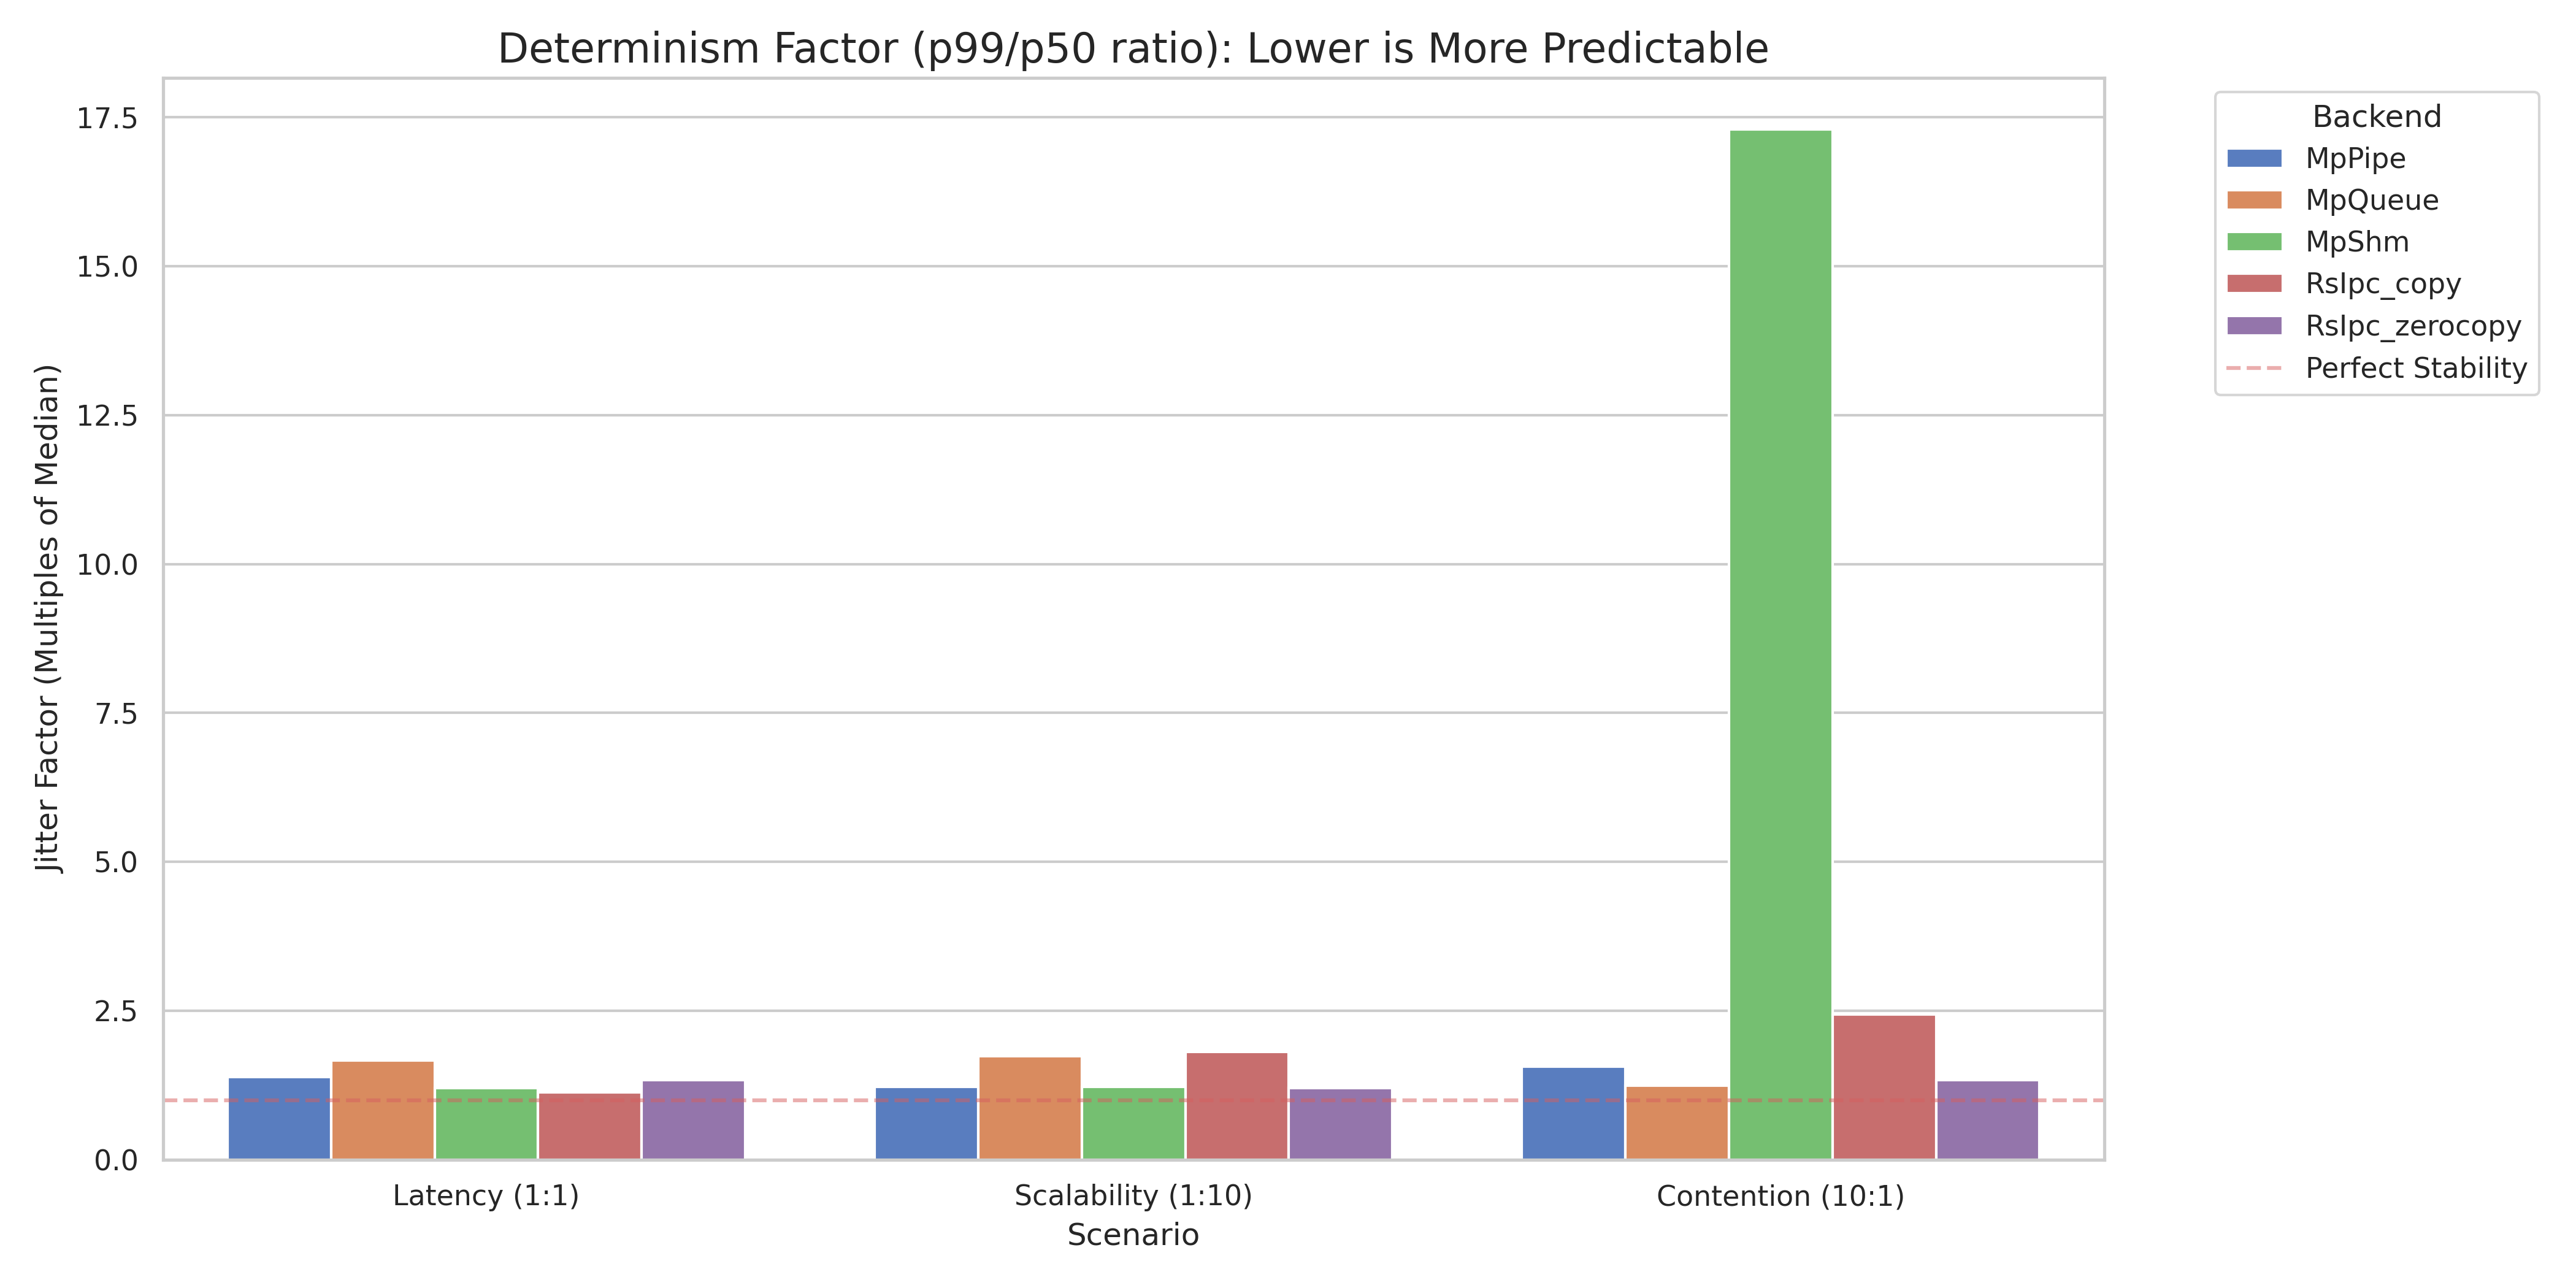
\includegraphics[width=\textwidth]{./figures/02_determinism.png}
    \caption{Determinism factor (p99/p50 ratio) across scenarios. A ratio of 1.0 represents perfectly predictable latency. RsIpc (zerocopy) maintains a ratio below 1.4 in all scenarios, while MpShm degrades to 17.3$\times$ under contention.}
    \label{fig:determinism}
\end{figure}

RsIpc (zerocopy) demonstrates the most consistent behavior, maintaining a determinism ratio below 1.4 across all three scenarios. This stability stems from the futex-based synchronization: the combination of spin-waiting (up to 1000 iterations in \texttt{SharedCondvar}) and direct kernel notification via \texttt{futex\_wake\_all} ensures bounded wakeup latency regardless of contention level.

RsIpc (copy) exhibits higher variance under contention (2.43$\times$) due to the interaction between multiple writers contending for the \texttt{FutexLock} and the three-state lock protocol. When the lock transitions to the \texttt{CONTENDED} state, waiting writers must perform a futex system call, introducing kernel scheduling latency. Nevertheless, this remains well below the 17.3$\times$ ratio observed with MpShm.

For real-time applications, predictable latency is often more critical than minimal average latency. A system with p50 = 2~ms and p99 = 3~ms (ratio 1.5) is preferable to one with p50 = 1~ms and p99 = 35~ms (ratio 35) because the former permits tighter deadline budgeting.

\subsection{Throughput and Efficiency}
\label{subsec:throughput_results}

Figure~\ref{fig:efficiency} shows the efficiency score (throughput in MB/s divided by median latency in ms) for each backend and scenario.

\begin{figure}[htbp]
    \centering
    
\includegraphics[width=\textwidth]{./figures/03_efficiency.png}
    \caption{Architectural efficiency: throughput (MB/s) per millisecond of median latency. Higher values indicate better utilization of the available bandwidth relative to synchronization cost. RsIpc (copy) dominates in the 1:1 scenario due to its minimal lock hold time.}
    \label{fig:efficiency}
\end{figure}

In the 1:1 scenario, RsIpc (copy) achieves 25,886~MB/s throughput---equivalent to approximately 25.3~GB/s, approaching the theoretical DDR5 memory bandwidth of the test system. This result demonstrates that the synchronization overhead (futex lock acquisition, sequence increment) is negligible compared to the \texttt{memcpy} cost: a single 2.76~MB copy completes in under 200~\textmu s.

In the scalability scenario (1:10), RsIpc (zerocopy) achieves the highest throughput (2,513~MB/s) among all backends. This advantage arises because the zerocopy mode allows multiple readers to access shared memory concurrently without requiring per-reader copies, while the copy mode must serialize each reader's access through the write lock (since the write overwrites the shared buffer). The throughput advantage of RsIpc over \texttt{multiprocessing.Queue} (5.3$\times$) and \texttt{multiprocessing.Pipe} (7.3$\times$) in this scenario reflects the fundamental overhead of pipe-based communication: each message must traverse the kernel pipe buffer for each reader independently.

\subsection{Message Size Scaling}
\label{subsec:size_scaling_results}

Table~\ref{tab:size_scaling} presents throughput across message sizes for the 1:1 scenario, and Figure~\ref{fig:size_scaling} visualizes the scaling behavior.

\begin{table}[htbp]
    \centering
    \caption{Throughput (MB/s) by message size in the 1:1 scenario.}
    \label{tab:size_scaling}
    \begin{tabular}{lrrrrr}
        \hline
        \textbf{Size} & \textbf{RsIpc (zc)} & \textbf{RsIpc (cp)} & \textbf{MpQueue} & \textbf{MpPipe} & \textbf{MpShm} \\
        \hline
        1~MB  & 21,014 & 3,341 & 2,323 & 3,624 & 3,150 \\
        2~MB  & 23,283 & 3,396 & 1,856 & 3,746 & 3,305 \\
        4~MB  & 26,246 & 19,378 & 2,328 & 3,693 & 18,200 \\
        8~MB  & 25,975 & 14,974 & 2,339 & 3,819 & 18,566 \\
        16~MB & 17,814 & 7,676 & 2,313 & 3,644 & 10,312 \\
        32~MB & 3,449 & 2,322 & 1,533 & 1,560 & 3,427 \\
        \hline
    \end{tabular}
\end{table}

\begin{figure}[htbp]
    \centering
    
\includegraphics[width=\textwidth]{./figures/04_size_scaling.png}
    \caption{Throughput versus message size (1:1 scenario, log-scale x-axis). RsIpc (zerocopy) maintains superior throughput up to 16~MB before degrading at 32~MB as the working set exceeds L3 cache capacity.}
    \label{fig:size_scaling}
\end{figure}

Three distinct regimes emerge from the size-scaling data:

\textbf{Small messages (1--2~MB)}: RsIpc (zerocopy) achieves 21,000--23,000~MB/s, far exceeding all other backends. At these sizes, the entire message fits within the L3 cache, and the zerocopy path---which writes directly into shared memory without an intermediate buffer---avoids the cache pollution that a temporary allocation would cause. MpPipe and MpQueue maintain consistent but low throughput (2,300--3,700~MB/s), bounded by kernel pipe buffer management overhead.

\textbf{Medium messages (4--8~MB)}: Both RsIpc (zerocopy) at 26,000~MB/s and the shared-memory-based backends (RsIpc copy, MpShm) at 14,000--19,000~MB/s achieve high throughput. The working set still fits within the L3 cache (32~MiB), enabling efficient streaming from the write buffer. MpPipe and MpQueue remain capped by kernel copy overhead.

\textbf{Large messages (16--32~MB)}: Performance degrades sharply for all shared-memory backends. At 32~MB, the working set equals the L3 cache size, causing cache thrashing: the write and read of a single message evict the entire cache contents. RsIpc (zerocopy) and MpShm converge to similar throughput (3,427--3,449~MB/s), as both reduce to a single \texttt{memcpy}-equivalent operation bounded by DRAM bandwidth. Pipe-based mechanisms (MpQueue, MpPipe) degrade further due to additional kernel-mediated copies.


\section{Analysis: Copy vs.\ Zero-Copy Trade-off}
\label{sec:copy_vs_zerocopy}

The benchmark results reveal a counterintuitive finding: the ``copy'' mode of \texttt{rs\_ipc} consistently outperforms the ``zerocopy'' mode in latency for pickle-based workloads (0.19~ms vs.\ 0.84~ms in the 1:1 scenario). This section analyzes the root cause and identifies the conditions under which each mode is optimal.

\subsection{Critical Section Analysis}

The fundamental difference between the two modes lies in their lock hold duration. Table~\ref{tab:critical_section} summarizes the execution paths.

\begin{table}[htbp]
    \centering
    \caption{Critical section comparison between copy and zerocopy modes.}
    \label{tab:critical_section}
    \begin{tabular}{lll}
        \hline
        \textbf{Phase} & \textbf{Copy Mode} & \textbf{Zerocopy Mode} \\
        \hline
        1. Serialize & \texttt{pickle.dumps(obj)} & (deferred to step 3) \\
          & $\sim$800~\textmu s, no lock held & \\
        2. Acquire lock & \texttt{start\_write()} & \texttt{write\_guard()} \\
          & via \texttt{FutexLock} & via \texttt{FutexLock} \\
        3. Transfer data & single \texttt{memcpy} & \texttt{pickle.dump(obj, guard)} \\
          & $\sim$2~\textmu s & $\sim$800~\textmu s, hundreds of \\
          & & incremental \texttt{.write()} calls \\
        4. Publish & sequence increment & sequence increment \\
        5. Release lock & drop guard & drop guard \\
        \hline
        \textbf{Lock hold time} & $\sim$2~\textmu s & $\sim$800~\textmu s \\
        \hline
    \end{tabular}
\end{table}

In copy mode, serialization occurs entirely outside the critical section. The writer calls \texttt{pickle.dumps(obj)} to produce a byte string in the Python heap (approximately 800~\textmu s for a 2.76~MB payload), then acquires the writer mutex and performs a single \texttt{ptr::copy\_nonoverlapping} to transfer the pre-serialized data into shared memory. The lock is held for approximately 2~\textmu s---just the duration of one \texttt{memcpy}.

In zerocopy mode, the writer first acquires the lock via \texttt{write\_guard()}, then calls \texttt{pickle.dump(obj, guard)}. The pickle protocol serializes the object through hundreds of incremental \texttt{.write()} calls to the guard's buffer protocol interface. Each call crosses the Python-to-Rust FFI boundary, performs a bounds check, and executes a small \texttt{memcpy} into shared memory. The lock is held throughout this entire process---approximately 800~\textmu s.

The ratio of lock hold times is approximately 400$\times$, which directly impacts contention: in multi-reader scenarios, readers must wait for the writer to release the mutex before accessing updated data.

\subsection{When Each Mode Excels}

Despite its higher latency in pickle-based workloads, the zerocopy mode offers advantages in specific use cases:

\begin{itemize}
    \item \textbf{Pre-serialized data}: When the payload is already a contiguous byte buffer (e.g., a raw NumPy array or a pre-encoded video frame), the zerocopy write path performs a single large \texttt{memcpy} identical to copy mode, but avoids allocating a temporary buffer. The size-scaling results confirm this: at 1~MB with raw byte payloads, RsIpc (zerocopy) achieves 21,014~MB/s versus 3,341~MB/s for copy mode.

    \item \textbf{Memory-constrained environments}: Copy mode requires allocating a temporary buffer equal to the serialized message size. For large payloads or systems with limited memory headroom, zerocopy eliminates this allocation entirely.

    \item \textbf{Fan-out patterns}: In the 1:10 scalability scenario, zerocopy achieves 1.85$\times$ higher throughput than copy mode (2,513 vs.\ 1,602~MB/s). Multiple readers can access the shared memory region concurrently through read guards, whereas copy mode incurs per-reader overhead.
\end{itemize}

The recommendation for application developers is clear: use copy mode for pickle-based workloads where latency is the primary concern, and zerocopy mode for pre-serialized data (raw arrays, encoded frames) or memory-constrained multi-reader scenarios where throughput dominates.


\section{Comparison with External IPC Libraries}
\label{sec:external_ipc}

A comprehensive comparison with external IPC libraries beyond Python's standard library is planned as future work. The following systems are targeted for evaluation:

\begin{itemize}
    \item \textbf{ZeroMQ}: Using PAIR sockets with the IPC transport, representing a mature general-purpose messaging library with batching and zero-copy optimizations.
    \item \textbf{nanomsg / nng}: A lightweight messaging library with similar socket abstractions but simpler internals.
    \item \textbf{Unix domain sockets}: Raw socket communication without a messaging framework, establishing the baseline for kernel-mediated IPC.
    \item \textbf{Rust ipc-channel}: Mozilla's Rust-native IPC library, evaluating the overhead of a Rust-to-Rust path through Python bindings.
\end{itemize}

These comparisons will use the same methodology described in Section~\ref{sec:bench_methodology}, with the 2.76~MB payload and both the 1:1 and 1:10 scenarios as primary evaluation points. The focus will be on latency and throughput positioning: \texttt{rs\_ipc} targets a niche between raw shared memory (maximum performance, no safety) and general-purpose messaging (convenience, higher overhead).


\section{Rust-Level Microbenchmarks}
\label{sec:rust_microbench}

To isolate the cost of the Rust synchronization layer from Python/PyO3/pickle overhead, Criterion microbenchmarks measure raw write throughput at the Rust level using a 1~MB payload.

\subsection{Benchmark Configuration}

Three benchmark functions evaluate different synchronization costs:

\begin{itemize}
    \item \textbf{\texttt{pure\_write}}: Writes 1~MB to shared memory with \texttt{target\_read\_count = 0} and no registered readers. Measures the raw write path: mutex acquisition, \texttt{memcpy}, sequence increment, mutex release.

    \item \textbf{\texttt{write\_no\_wait\_with\_reader}}: Same configuration as \texttt{pure\_write}, but with one registered reader consuming messages on a background thread. The writer does not wait for consumption (\texttt{target\_read\_count = 0}), so this measures the cost of concurrent reader access on the write path.

    \item \textbf{\texttt{write\_waiting\_with\_N\_readers}}: Configures \texttt{target\_read\_count = N} with $N$ active reader threads. The writer blocks in \texttt{start\_write()} until all $N$ readers have consumed the previous message. This measures the full synchronization cost including condvar signaling and wakeup latency.
\end{itemize}

Each benchmark uses Criterion's default configuration with 50 samples and 2-second measurement windows per sample.

\subsection{Expected Scaling Behavior}

The write-with-readers benchmarks reveal the synchronization cost as a function of reader count. With \texttt{target\_read\_count = N}, the writer must wait for the \texttt{data\_consumed} counter (packed in the \texttt{ReadersStateCount} atomic, as described in Chapter~\ref{chap:ch4}) to reach $N$ before proceeding. Each reader increments this counter upon completing its read, triggering a \texttt{futex\_wake\_all} on the writer's condvar.

The expected latency increase per additional reader is bounded by:
\begin{enumerate}
    \item The read duration (1~MB \texttt{memcpy} $\approx$ 100--200~\textmu s per reader, parallelized across cores).
    \item One \texttt{futex\_wake} system call per reader completion ($\approx$ 1~\textmu s each).
    \item The writer's spin-wait or \texttt{futex\_wait} to observe the counter update.
\end{enumerate}

Since readers operate concurrently, the total wait time scales with the slowest reader rather than the sum of all readers---a consequence of the partial-blocking design described in Section~\ref{sec:sync} of Chapter~\ref{chap:ch2}. However, cache contention on the \texttt{ReadersStateCount} atomic increases linearly with reader count due to the MESI invalidation traffic described in Section~\ref{subsec:false_sharing} of Chapter~\ref{chap:ch2}.


\section{Discussion}
\label{sec:bench_discussion}

\subsection{Where rs\_ipc Excels}

The benchmark results identify three areas of clear advantage for \texttt{rs\_ipc}:

\textbf{Multi-reader scalability}: In the 1:10 scenario, RsIpc (zerocopy) achieves 5.3$\times$ higher throughput than \texttt{multiprocessing.Queue} and 4.8$\times$ higher than MpShm. The lock-free version checking mechanism (described in Chapter~\ref{chap:ch4}) allows readers to detect new messages without acquiring any lock, reducing contention on the critical path.

\textbf{Tail latency predictability}: RsIpc maintains determinism ratios below 2.5$\times$ in all scenarios, while MpShm degrades catastrophically (17.3$\times$) under writer contention. The futex-based synchronization provides bounded wakeup latency that Python's condition variable polling cannot match.

\textbf{Large payload throughput}: For pre-serialized data in the 4--8~MB range, RsIpc (zerocopy) achieves 25,000--26,000~MB/s---approximately 7$\times$ higher than pipe-based mechanisms and 1.4$\times$ higher than MpShm.

\subsection{Limitations}

\textbf{Copy mode paradox}: For pickle-based workloads, the ``copy'' mode outperforms ``zerocopy'' in latency because pickle serialization holds the writer mutex for the entire serialization duration in zerocopy mode. This is inherent to the buffer-protocol approach and cannot be resolved without changing the pickle protocol or pre-serializing data.

\textbf{32~MB degradation}: At payload sizes equal to or exceeding the L3 cache (32~MiB), all shared-memory backends converge to similar performance, bounded by DRAM bandwidth. The synchronization advantages of \texttt{rs\_ipc} become irrelevant when memory subsystem throughput is the bottleneck.

\textbf{Platform restriction}: The futex-based synchronization is Linux-specific. Portability to other operating systems would require alternative synchronization backends (e.g., Windows \texttt{WaitOnAddress}, macOS \texttt{os\_unfair\_lock}), potentially with different performance characteristics.

\subsection{Implications for System Design}

The results suggest the following guidelines for developers choosing an IPC strategy:

\begin{enumerate}
    \item For single-producer, single-consumer pipelines with pickle-based data: \texttt{rs\_ipc} copy mode offers 7$\times$ lower latency than \texttt{multiprocessing.Queue} with minimal API complexity.

    \item For fan-out architectures (one camera, multiple consumers): \texttt{rs\_ipc} zerocopy mode provides the best combination of throughput and predictability, with the added benefit of concurrent reader access.

    \item For latency-critical paths with raw byte data (pre-encoded frames, NumPy arrays): \texttt{rs\_ipc} zerocopy mode achieves true zero-copy semantics with throughput approaching memory bandwidth limits.

    \item When predictable worst-case latency matters more than average performance: \texttt{rs\_ipc}'s determinism advantage (1.2--1.4$\times$ ratio vs.\ up to 17$\times$ for MpShm) enables tighter deadline budgets in real-time systems.
\end{enumerate}


\chapter{Conclusions}
\label{chap:conclusions}

% TODO: Highlight that the ReaderWaitPolicy abstraction extends beyond shared-memory
% blocking behavior to fundamentally change the system's delivery semantics. Combined
% with WriteAsync, the same library serves as both a real-time data bus (latest-value,
% lossy via Count(0)) and a reliable message queue (ordered, guaranteed delivery via
% All()), selected at construction time without architectural changes.


\addcontentsline{toc}{chapter}{Conclusions}

\bibliography{references}

\end{document}
